\parindent=0em
\subsection{HMD Odyssey+}
\noindent

%https://www.samsung.com/us/computing/hmd/windows-mixed-reality/hmd-odyssey-windows-mixed-reality-headset-xe800zba-hc1us/

El casco \textit{HDM Odyssey+} es un dispositivo desarrollado por la empresa Samsung que salió al mercado el 22 de Octubre de 2018, destaca por su sonido espacial que abarca los 360 grados y su campo de visión de 110 grados.\\

\begin{figure}[h]
    \centering
    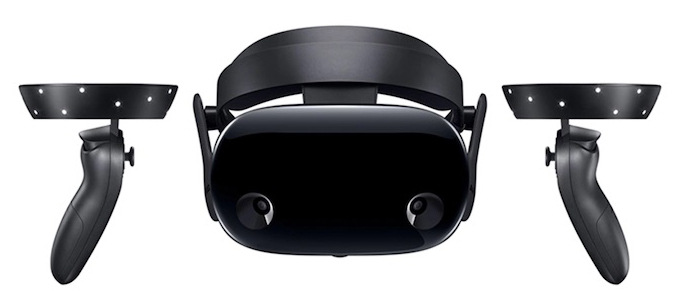
\includegraphics[scale=0.5]{Images/Estado del arte/samsungOdysseyplus.jpg}
    \caption{HDM Odyssey+ dispositivo al completo.}
    \label{fig:hdmOdysseyVista}
\end{figure}

Este dispositivo está dotado de varios sensores: Giroscopio, brújula de tres ejes, sensor de proximidad y sensor IPD (distancia interpupilar). Por otro lado, tiene dos cámaras 6DOF y un peso considerablemente superior a otros dispositivos de 590 gramos, además, almacena un total de 10 Gigabytes.\\

Ya que esta diadema está enfocada para las plataformas de 	Windows MR y Steam VR support, necesita unos requerimientos mínimos en el ordenador que las utilice. Estos requerimientos son, entre otros, 8 Gigabytes DDR3 de memoria RAM(memoria de acceso aleatorio), al menos 10 Gigabytes de espacio en disco y una CPU Intel Core i5 4590 (cuarta generación) o AMD Ryzen 5 1400 a 3.4 Gigahercios. El precio actual del dispositivo es de 279 dólares.


\footnotetext[1]{
\label{hdmOdysseyfooter}{Imagen de la HDMOdyssey+: \url{https://www.samsung.com/us/computing/hmd/windows-mixed-reality/hmd-odyssey-windows-mixed-reality-headset-xe800zba-hc1us/}.}}

\footnotetext[1]{
\label{hdmOdysseyfooter}{Especificaciones de la HDMOdyssey+: \url{https://www.microsoft.com/en-us/p/samsung-hmd-odyssey/8n2d0nk20p8m?cid=msft_web_collection&activetab=pivot:techspecstab}.}}